\section{Computational Simulation}

\subsection{Theoretical Background}

\subsubsection{Samara Autorotation}

The SRAB is inspired by the autorotation of samara seeds (\emph{Acer
rubrum}). The seed geometry places the center of mass at one end and
the aerodynamic center at the other, generating a torque imbalance
that produces stable conical rotation during fall. The resulting
motion is a steady autorotation state where the descent rate is
substantially lower than the ballistic terminal velocity of the same
mass [\ref{ref2}].

\subsubsection{Leading-Edge Vortex (LEV)}

At high incidence angles and rotation rates, a stable leading-edge
vortex forms on the wing upper surface, increasing the effective lift
coefficient beyond the thin-airfoil limit. This LEV effect is the key
to the samara's efficiency and is modeled through an augmented lift
coefficient in the blade element formulation.

\subsubsection{Reduced-Order Rigid-Body Model}

The descent is modeled with a 4th-order reduced Newton-Euler
formulation [\ref{ref3}], with state vector (Eq.~\ref{eq:state}):

\begin{equation}
\mathbf{x} = [\theta,\ \dot{\theta},\ \dot{\phi},\ v_0]^T
\label{eq:state}
\end{equation}

where $\theta$ is the conicity angle, $\dot{\phi}$ the rotor spin rate
and $v_0$ the vertical descent velocity. The aerodynamic loads are
computed with the Blade Element Method (BEM) (Eq.~\ref{eq:bem}):

\begin{equation}
dF = \frac{1}{2}\rho\, w(r)\, \|U\|^2 \left[C_L(\alpha),\; C_D(\alpha)\right] dr
\label{eq:bem}
\end{equation}

with the thin-airfoil lift curve and the induced-drag model
(Eq.~\ref{eq:coefs}):

\begin{equation}
C_L = 2\pi\sin\alpha, \qquad
C_D = C_L \sin\alpha + C_{D0}
\label{eq:coefs}
\end{equation}

where $C_{D0} = 1.0$ is the flat-plate drag coefficient and the LEV
contribution is embedded through the $f_{factor} = 0.3$ correction in
the lift build-up [\ref{ref4}].

\subsection{Simulation Methodology}

The validation pipeline is an iterative loop: model, simulate,
prototype, drop, compare, and iterate on the geometry. PETG
3D-printed wings (Asa1, Asa2 and Asa3 geometries) are dropped from
controlled heights with instrumentation, and the measured terminal
velocity, spin rate and cone angle are compared against the
simulation. The wing geometry is updated between test cycles based
on that comparison, which is how the design improved from one
campaign to the next. The simulation itself is implemented in
RocketPy~[\ref{ref6}] with a custom SRAB extension module, as
described in the next subsection.

\subsubsection{Coupling the SRAB Descent to the RocketPy Ascent}

The launch vehicle is simulated in RocketPy using a standard
\texttt{Flight} with \texttt{terminate\_on\_apogee=True}, which
stops the integration at the apogee state (altitude, position,
velocity) of the Dédalo stage with payload. The descent is then
modelled with a separate, dedicated ODE solver that consumes the
apogee state as initial conditions --- the SRAB is \emph{not} a
\texttt{rocketpy.Rocket} because its autorotation dynamics cannot
be expressed as \texttt{add\_parachute()}:

\begin{itemize}
  \item Wing geometry is loaded from the \texttt{Asa3.DXF} CAD file
    into a \texttt{PocketQubeSamaraWing} object
    (\texttt{n\_wings=2}, $\beta = 5.0^{\circ}$); the aerodynamic
    radius is then \emph{optimised} inside the \texttt{SRABRecovery}
    constructor to bring the impact velocity to the target
    $V_F^{target} = V_{F,\max}/\mathrm{FS} = 13.33$~m/s (Table~\ref{tab:srab-descent}).
  \item The descent ODE is integrated by
    \texttt{EnvironmentAwareFlightDynamics}, which extends the
    base dynamics class to query \texttt{env.density.get\_value\_opt(z)}
    at every step --- the descent therefore uses the same GFS
    atmospheric model as the ascent, not a constant $\rho$.
  \item Horizontal drift is integrated along the descent by
    sampling \texttt{env.wind\_velocity\_x/y.get\_value\_opt(z)} at
    each step, sharing the wind profile that drove the ascent
    through the Dédalo flight --- so the trajectory kink that
    appears around 1500--2000~m AGL in the descent plot is the
    same GFS shear layer the rocket crossed on the way up.
\end{itemize}

The result is a \emph{three-stage simulation}: Stage~1 (Dédalo
ascent with payload), Stage~2 (Dédalo descent without payload,
ballistic + parachute), and Stage~3 (PocketQube SRAB descent) ---
all three in the same atmosphere and same wind profile, with
apogee as the only hand-off point. The Dédalo ascent Flight is
reused as the SRAB solver's initial-condition source via
\texttt{simulate\_from\_flight(flight\_with\_payload)}, so any
change to the ascent parameters (mass, motor impulse, launch
angle) automatically propagates to the descent without manual
intervention.

\subsubsection{Launch Vehicle Model — Dédalo}

The Dédalo rocket (used as the launch vehicle for Helike) is
modeled in RocketPy, with the parameters summarized in
Table~\ref{tab:dedalo}:

\begin{table}[htbp]
\centering
{\small
\setlength{\tabcolsep}{6pt}
\begin{tabular}{>{\raggedright}p{5.2cm}l}
\toprule
\textbf{Parameter} & \textbf{Value} \\
\midrule
Total mass (with payload) & 5.100 kg \\
Empty mass (Stage 2) & 4.900 kg \\
Payload mass (Helike \#213) & 0.200 kg \\
Diameter & 106 mm \\
Motor & SolidMotor, 926 N peak, 2.82 s burn \\
Motor data points & 95 \\
Atmosphere & GFS (real, launch-day forecast) \\
Launch site & lat $-21.94305$, lon $-48.95409$, elev 478 m \\
\bottomrule
\end{tabular}
\caption{Dédalo \#11 simulation parameters.}
\label{tab:dedalo}

}
\end{table}

\subsection{Results}

\subsubsection{Dédalo Ascent (with payload)}

The simulated ascent of the Dédalo launch vehicle carrying the Helike
payload is summarized in Table~\ref{tab:flight}:

\begin{table}[htbp]
\centering
{\small
\setlength{\tabcolsep}{6pt}
\begin{tabular}{>{\raggedright}p{5.2cm}l}
\toprule
\textbf{Parameter} & \textbf{Value} \\
\midrule
Apogee & 1520 m AGL (1996 m ASL) \\
Time to apogee & 17.83 s \\
Maximum velocity & 205.3 m/s (0.59 Mach) \\
Maximum acceleration & 106.7 m/s$^2$ (10.9 g) \\
Rail departure & 0.47 s at 18.9 m/s \\
\bottomrule
\end{tabular}
\caption{Dédalo \#11 flight simulation results.}
\label{tab:flight}

}
\end{table}

\subsubsection{SRAB Descent from Real Apogee}

The SRAB simulation is initialized at the real apogee of Stage 1
(1520.5 m AGL, $v_z \approx 0$), with the optimized wing radius for
the target impact velocity $V_F^{target} = V_{F,max}/FS =
20/1.5 = 13.33$ m/s. The descent results are summarized in
Table~\ref{tab:srab-descent}, and the complete descent profile is
presented in the LRR certification dashboard
(Fig.~\ref{fig:lrr-asa3}), the satellite-view trajectory map
(Fig.~\ref{fig:trajectory-map}) and the full three-stage flight
trajectory (Fig.~\ref{fig:full-trajectory}):

\begin{table}[htbp]
\centering
{\small
\setlength{\tabcolsep}{6pt}
\begin{tabular}{>{\raggedright}p{5.2cm}l}
\toprule
\textbf{Parameter} & \textbf{Value} \\
\midrule
Wing geometry & Asa3 (2 wings), optimized radius 79.7 mm \\
Release altitude & 1520.5 m AGL \\
Impact velocity & 13.33 m/s \\
Descent time & 111.4 s \\
Equilibrium cone angle $\theta_{eq}$ & 8.6$^{\circ}$ \\
Impact spin rate & 477 RPM \\
Total drift & 184.3 m \\
Impact position (relative) & x $= -67.5$ m, y $= +171.5$ m \\
LASC descent criterion & Target $V_F = V_{F,max}/FS = 20/1.5 = 13.33$ m/s; simulated impact 13.33 m/s (PASS, FS 1.5) \\
\bottomrule
\end{tabular}
\caption{SRAB descent simulation results from real apogee.}
\label{tab:srab-descent}

}
\end{table}

\begin{figure}[htbp]
\centering
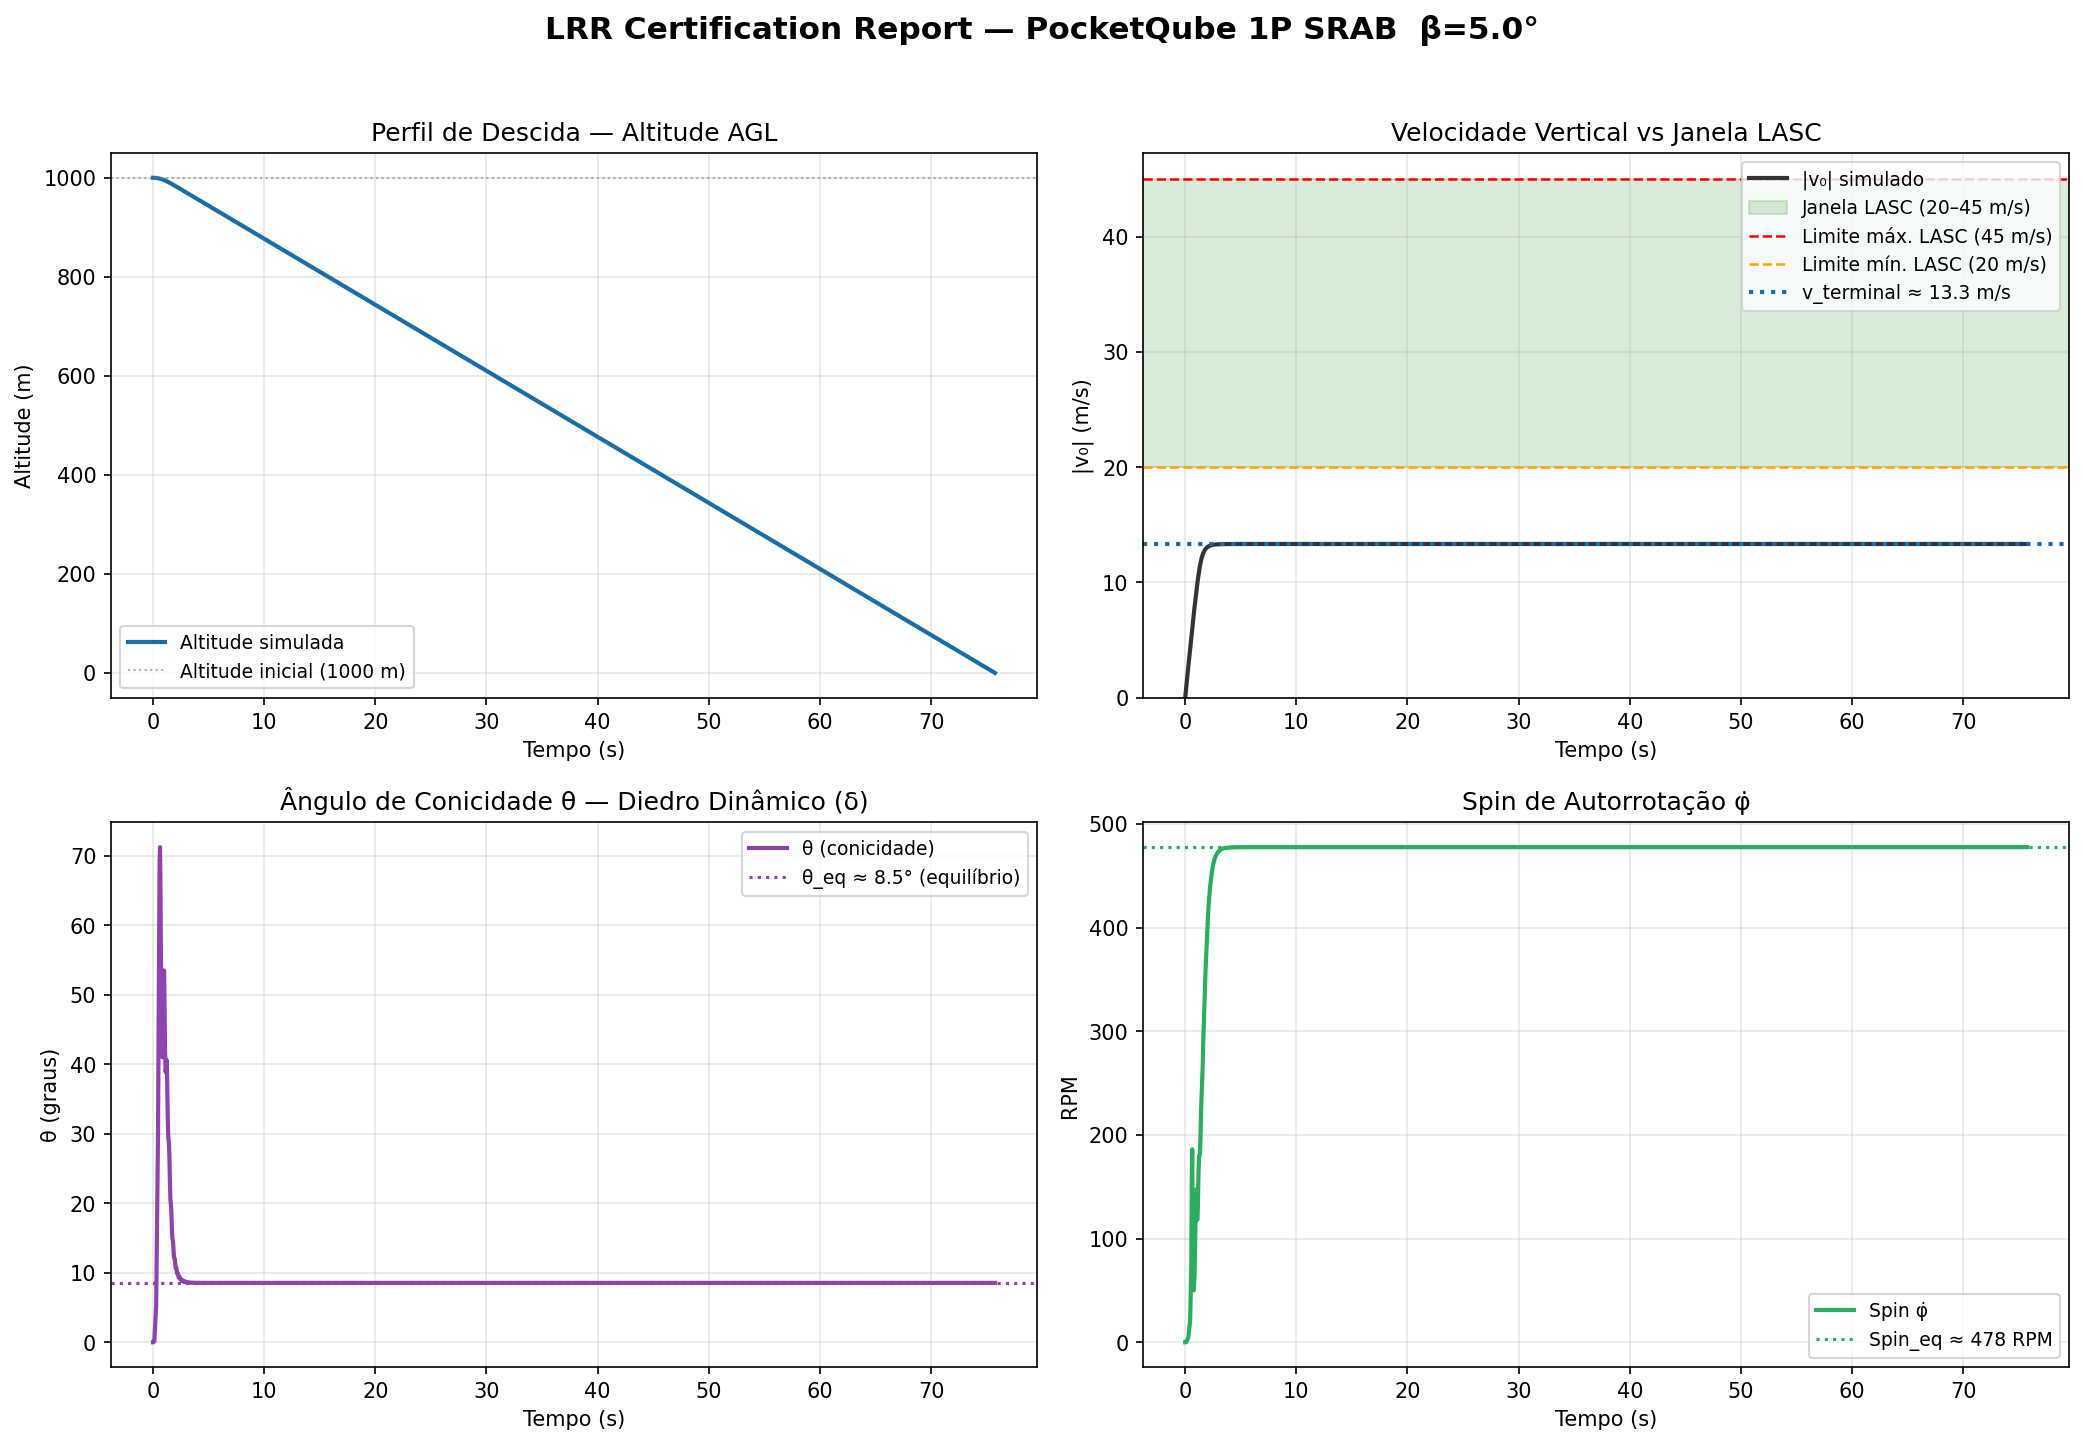
\includegraphics[width=0.9\textwidth]{figures/fig_asa3_lrr.png}
\caption{LRR certification dashboard for the SRAB descent from the
real apogee: altitude profile, vertical velocity, cone angle
$\theta$, and autorotation spin rate.}
\label{fig:lrr-asa3}
\end{figure}

\begin{figure}[htbp]
\centering
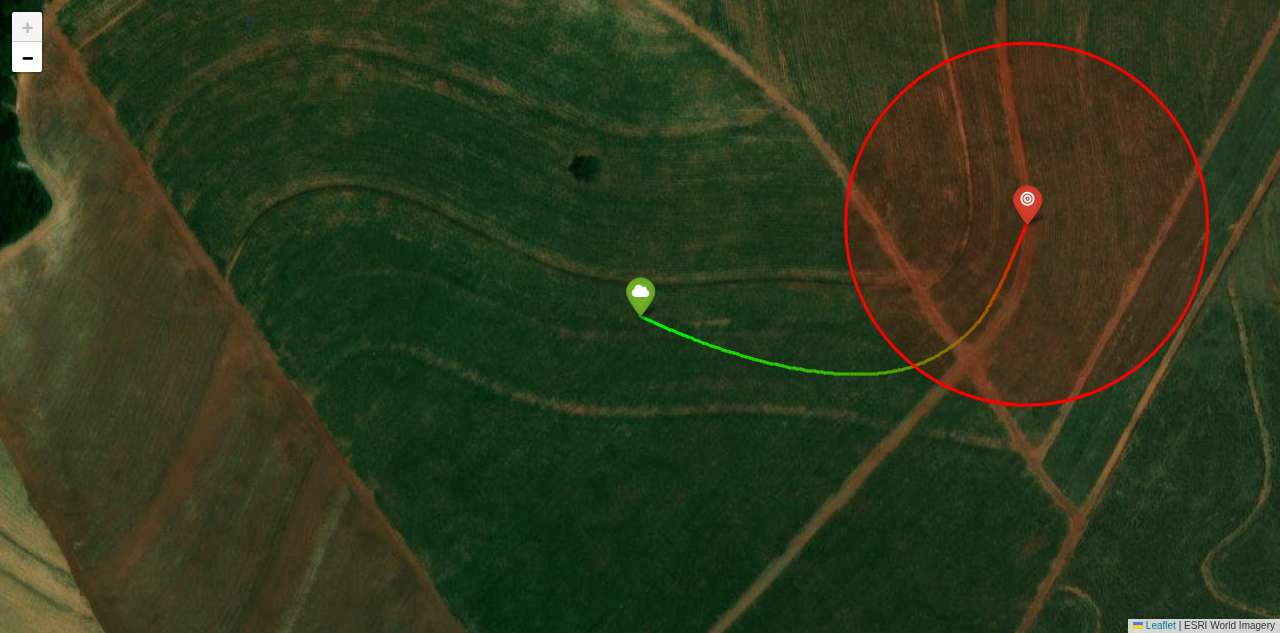
\includegraphics[width=0.9\textwidth]{figures/fig_trajectory_map.png}
\caption{Satellite view of the simulated SRAB descent trajectory over
the Dédalo launch site: release point (green marker) at apogee and
predicted impact point (red marker, 100~m radius circle) downrange;
the trajectory line is colored by altitude.}
\label{fig:trajectory-map}
\end{figure}

\begin{figure}[htbp]
\centering
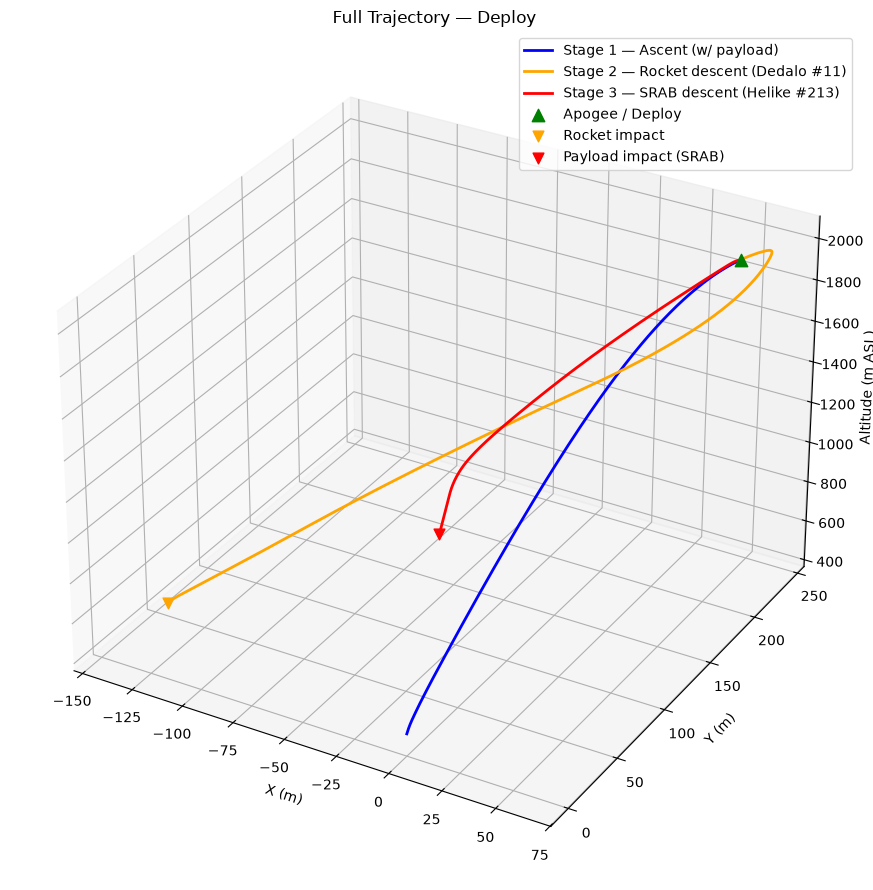
\includegraphics[width=0.9\textwidth]{figures/fig_full_trajectory.png}
\caption{Full simulated flight of the Dédalo launch vehicle carrying
the Helike payload: Stage 1 ascent with payload (blue), Stage 2 rocket
descent (orange) and Stage 3 SRAB descent (red), with the deployment
event at apogee and the two separate impact points.}
\label{fig:full-trajectory}
\end{figure}

\subsubsection{SRAB vs. Parachute Comparison}

A flat circular parachute ($\varnothing$200 mm, $C_D = 1.5$) was
simulated in the same GFS atmosphere, same release conditions and same
payload mass, as a benchmark. The comparison is summarized in
Table~\ref{tab:comparison}:

\begin{table}[htbp]
\centering
{\small
\setlength{\tabcolsep}{6pt}
\begin{tabular}{lrrr}
\toprule
\textbf{Parameter} & \textbf{SRAB} & \textbf{Parachute} & \textbf{Ratio} \\
\midrule
Impact velocity (m/s) & 13.33 & 8.48 & 1.57$\times$ \\
Descent time (s) & 111.4 & 174.6 & 0.64$\times$ \\
Total drift (m) & 131.2 & 204.6 & 0.64$\times$ \\
Impact energy (J) & 17.8 & 7.2 & 2.47$\times$ \\
Terminal velocity (SL) (m/s) & 13.33 & 8.24 & 1.62$\times$ \\
\bottomrule
\end{tabular}
\caption{SRAB vs.\ parachute comparison.}
\label{tab:comparison}

}
\end{table}

The SRAB achieves a 36\% shorter descent time and 36\% lower drift
than the parachute, at the cost of a higher impact velocity and
energy — both still well below the 20~m/s LASC limit. The shorter
descent reduces wind exposure (drift), which is the dominant factor
for recovery accuracy on miniaturized satellites.

\subsubsection{Monte Carlo Analysis}

A Monte Carlo analysis with 100 iterations of the Asa3 2-wing
configuration, released from the real simulated apogee, assessed
the descent under manufacturing and aerodynamic dispersion: the
impact velocity stayed at $13.33 \pm 0.31$~m/s (P5 12.78, P95
13.87), the descent time at $110.97 \pm 2.53$~s, the spin rate at
$475.9 \pm 12.8$~rpm and the equilibrium cone angle at
$8.63 \pm 0.67^{\circ}$ --- every iteration below the 20~m/s LASC
limit, confirming the 1.5 safety factor. The four parameters
varied are the manufacturing and mounting tolerances identified
during the Asa1$\rightarrow$Asa3 iteration: the payload mass
($\pm 10$~g, machining), the mounting pitch $\beta$ ($\pm
0.5^{\circ}$, assembly), and the two aerodynamic coefficients
($C_{D0}\pm 0.10$, $f_{factor}\pm 0.03$) which capture the BEM/LEV
calibration uncertainty against the 20~m drop data. $N = 100$
iterations are sufficient because the $v_{impact}$ dispersion is
dominated by the manufacturing parameters, which are themselves
tight --- the resulting $\sigma(v_{impact}) = 0.31$~m/s matches
the historical scatter observed across the 20~m drop campaigns.
The dispersion histograms of the three principal outputs are shown
in Fig.~\ref{fig:mc-sensitivity}:

\begin{figure}[htbp]
\centering
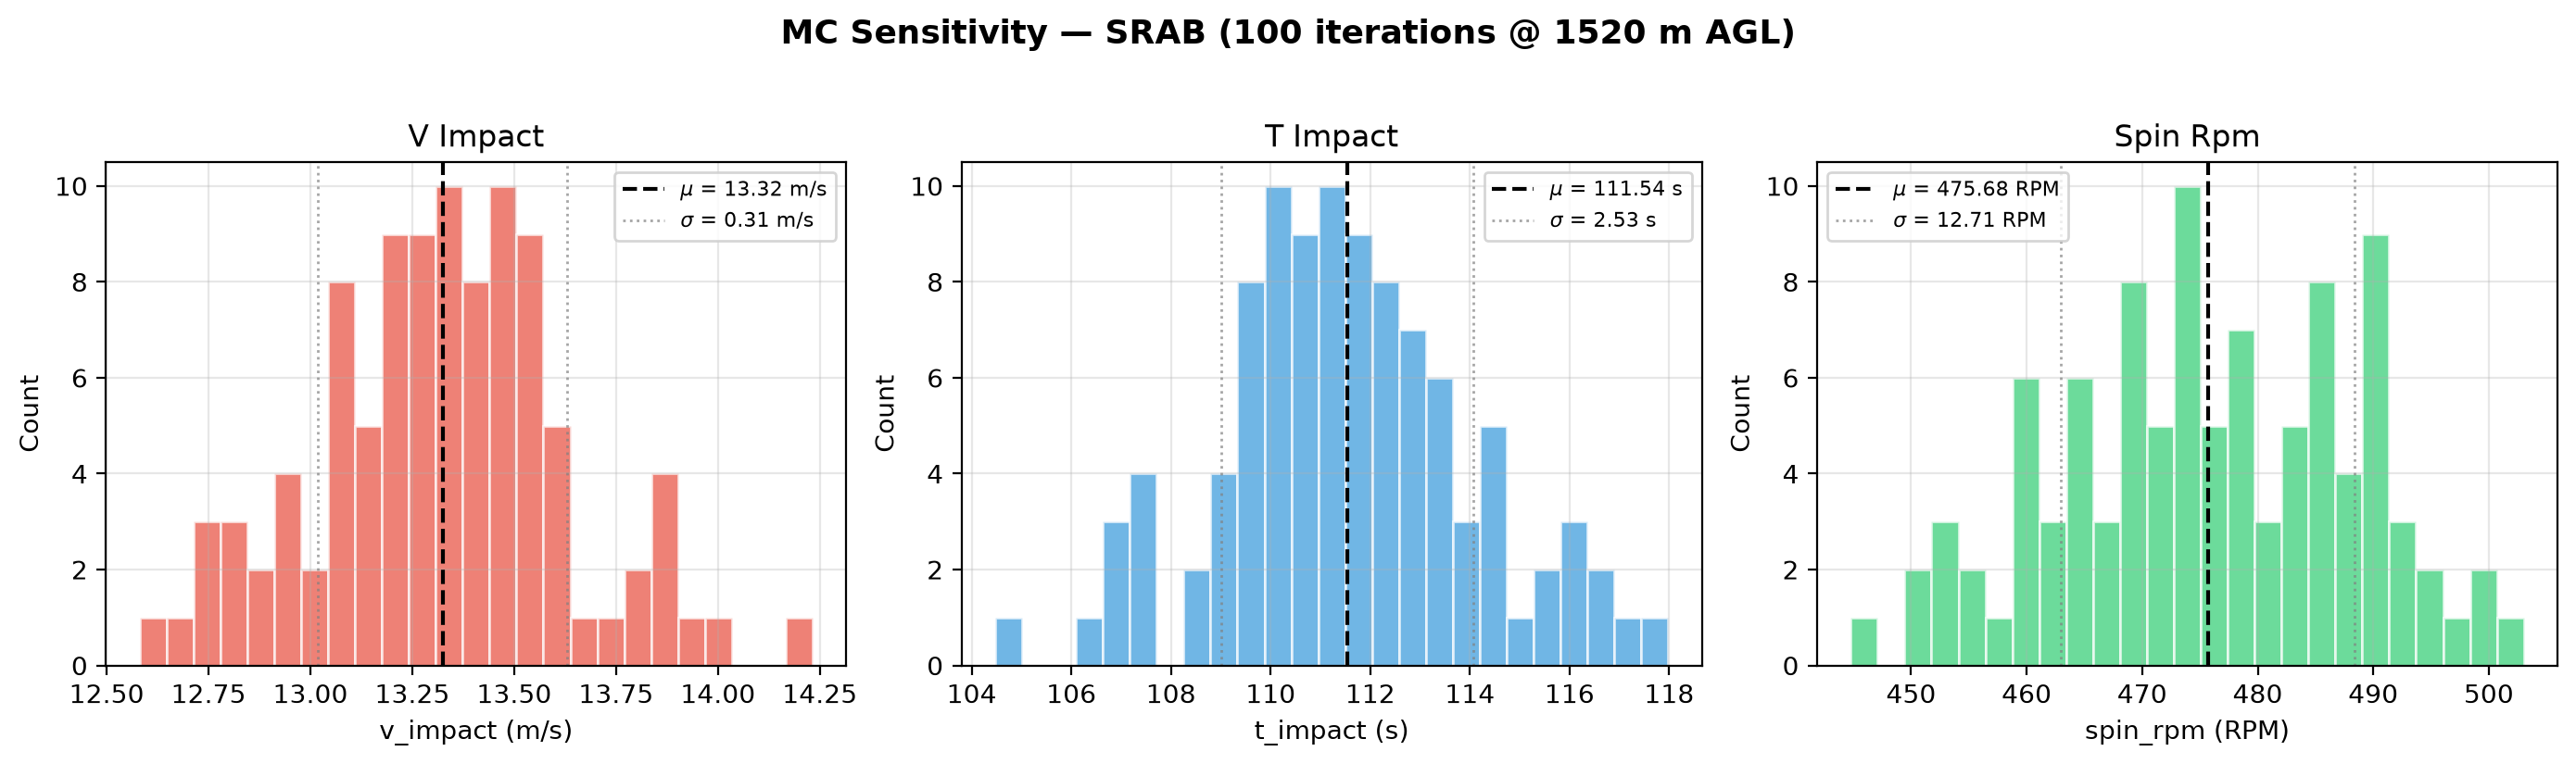
\includegraphics[width=0.9\textwidth]{figures/fig_mc_sensitivity.png}
\caption{Monte Carlo dispersion histograms (100 iterations, Asa3
2-wing, released from the real apogee): impact velocity (left),
descent time (center) and equilibrium spin rate (right). All
iterations remain below the 20~m/s LASC limit.}
\label{fig:mc-sensitivity}
\end{figure}

\subsubsection{Experimental Drop Tests}

Four instrumented drop-test campaigns validated the model: three
physical drops carried by a drone, plus the simulated 1000~m Test~3
that reuses the consolidated drone data through the 4th-order ODE
to extend the trajectory to the full descent regime. All physical
drops followed the same protocol --- a drone carried the prototype
to an altitude that was both safe for the surrounding area and
visually trackable from the ground station, released the
prototype at hover, and recorded the descent with the onboard
sensors. The wing geometries are designated \textbf{Asa1},
\textbf{Asa2}, and \textbf{Asa3} (Portuguese for ``wing'') in
chronological order of iteration. The results are summarised in
Table~\ref{tab:droptests}:

\begin{table}[htbp]
\centering
{\small
\setlength{\tabcolsep}{6pt}
\begin{tabular}{p{1.0cm}p{2.6cm}p{2.0cm}p{3.0cm}p{3.4cm}}
\toprule
\textbf{Test} & \textbf{Geometry} & \textbf{v impact} & \textbf{Spin / Cone} & \textbf{Setup / Notes} \\
\midrule
Test 1 & Asa1, 4 wings & 7.68~m/s & 306.8~rpm / 13.5$^{\circ}$ & Drone drop, $\sim$20~m; first observation of the autorotation principle \\
Test 2 & Asa2, 4 wings & 8.04~m/s & 306.9~rpm / 24.4$^{\circ}$ & Drone drop, $\sim$20~m; improved spin, alpha electronics validated --- demonstrated need for higher altitude to leave the transient regime \\
Test 3 & Asa3, 4 wings & 12.90~m/s & 372.0~rpm / 17.2$^{\circ}$ & Drone drop, $\sim$30~m, $\sim$200~g payload representative of the final assembly; electronics onboard \\
\bottomrule
\end{tabular}
\caption{Instrumented drop-test results. Tests~1--3 are physical
drops from a drone; the measured values were then extended through
the 4th-order SRAB ODE to the simulated 1000~m descent to reach
steady autorotation.}
\label{tab:droptests}
}
\end{table}

The certification dashboards of the two physical drop campaigns
(Test~1, Asa1 4-wing, and Test~2, Asa2 4-wing) are shown in
Fig.~\ref{fig:test1-lrr} and Fig.~\ref{fig:test2-lrr}:

\begin{figure}[htbp]
\centering
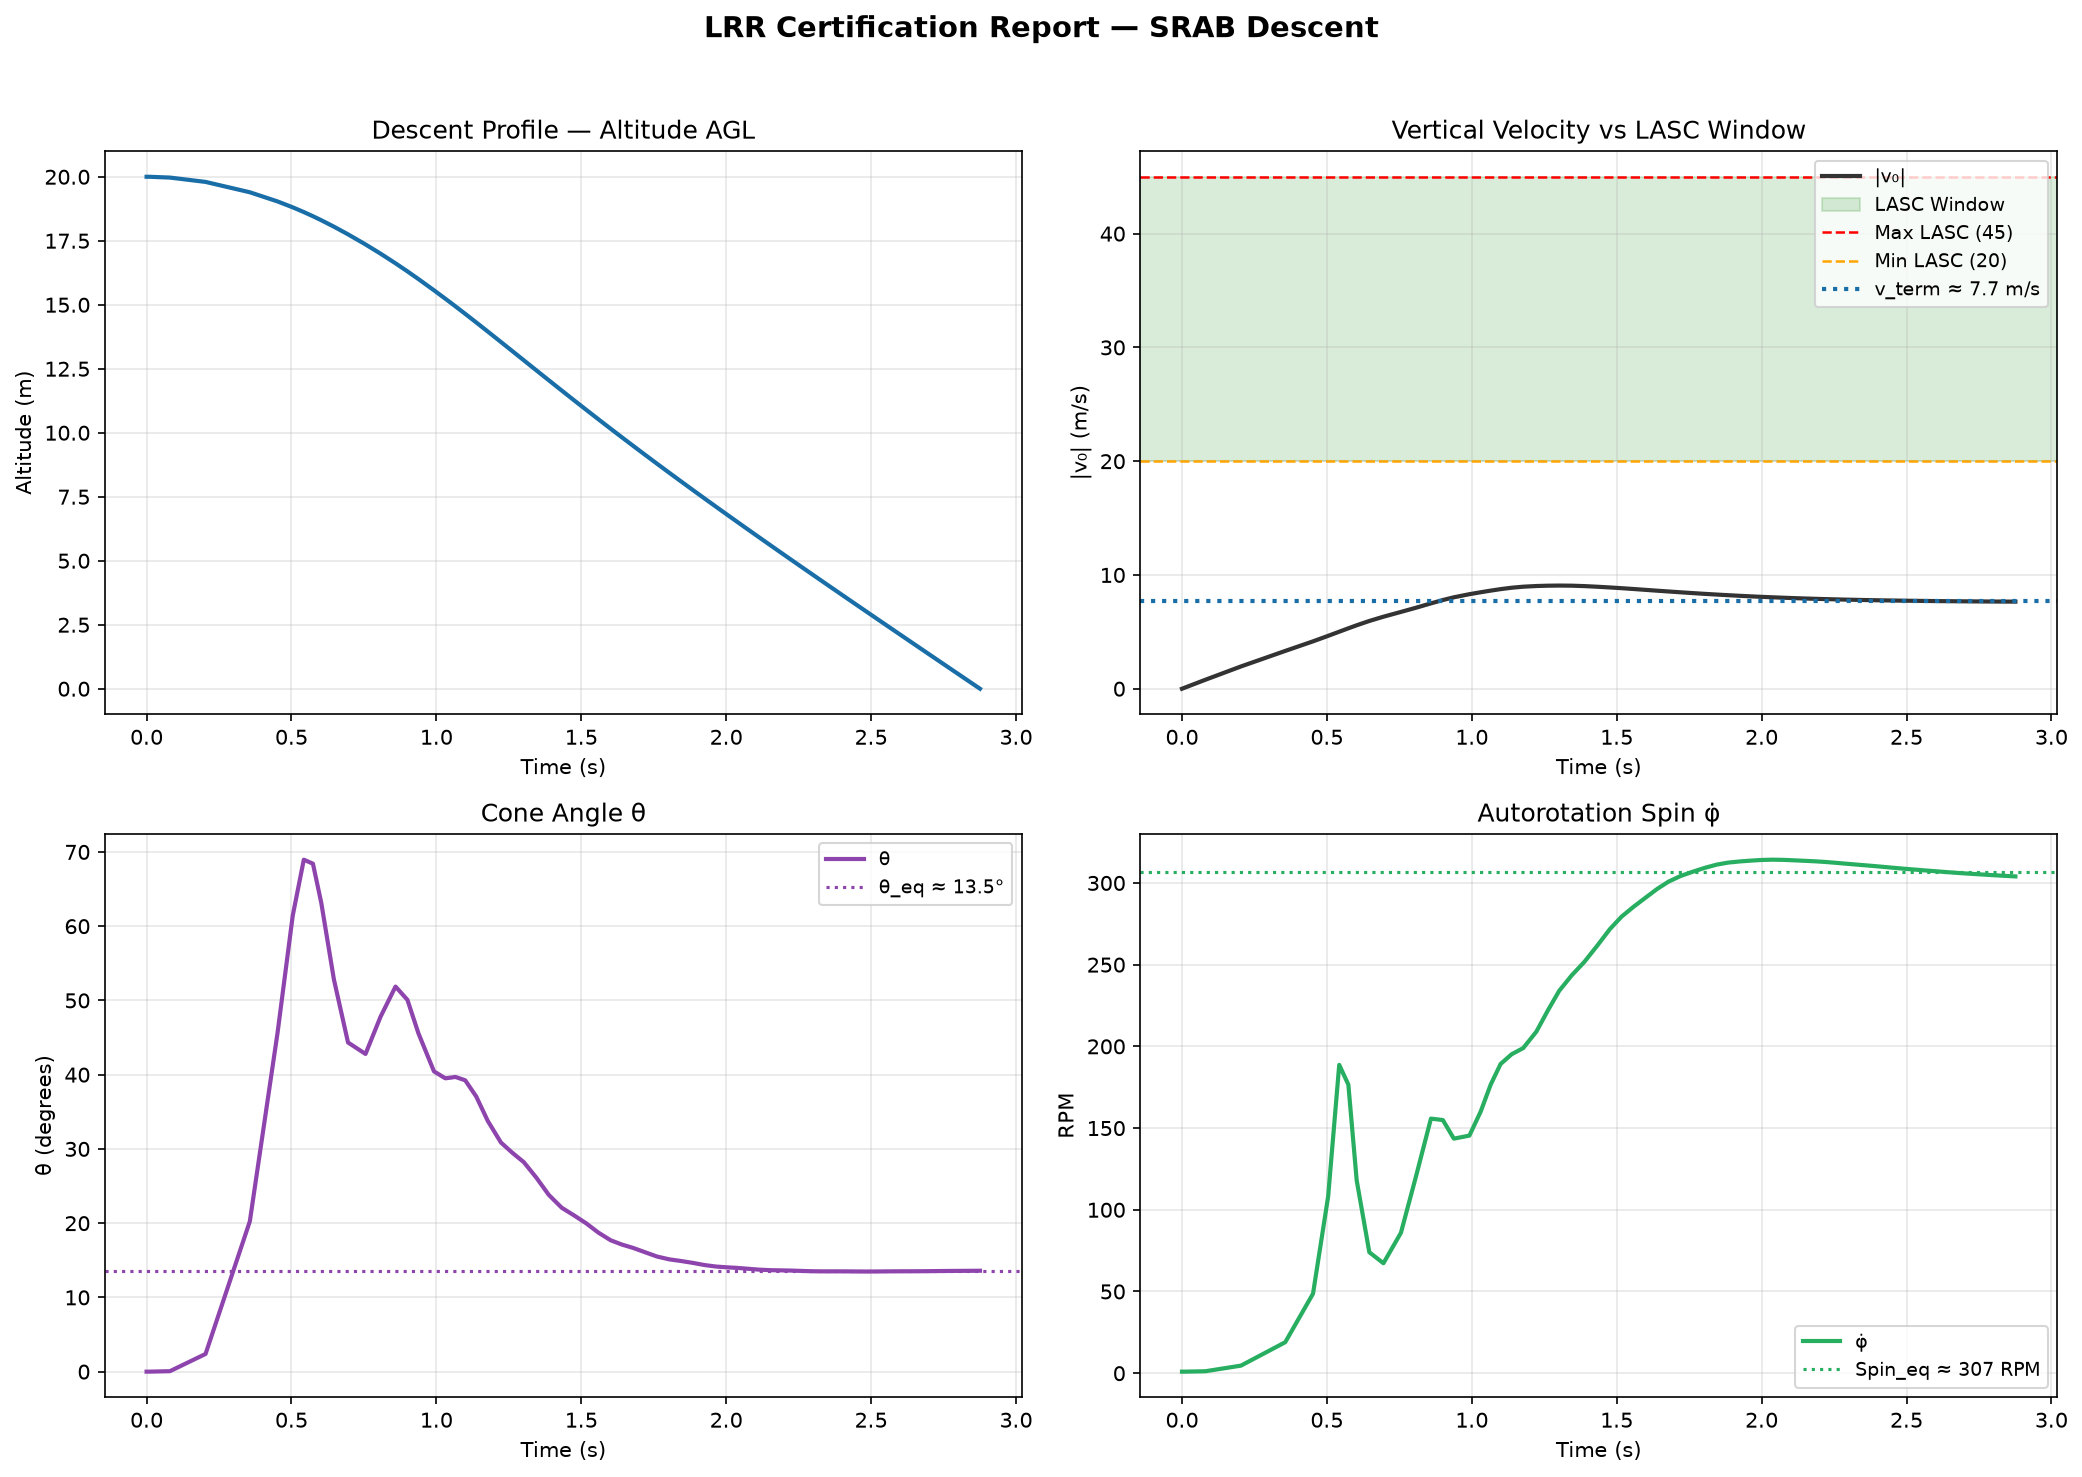
\includegraphics[width=0.9\textwidth]{figures/fig_test1_lrr.png}
\caption{LRR certification dashboard of Test~1 (Asa1, 4 wings, drone
drop from $\sim$20~m): altitude profile, vertical velocity against
the LASC window, cone angle and autorotation spin rate, converging
to the equilibrium values.}
\label{fig:test1-lrr}
\end{figure}

\begin{figure}[htbp]
\centering
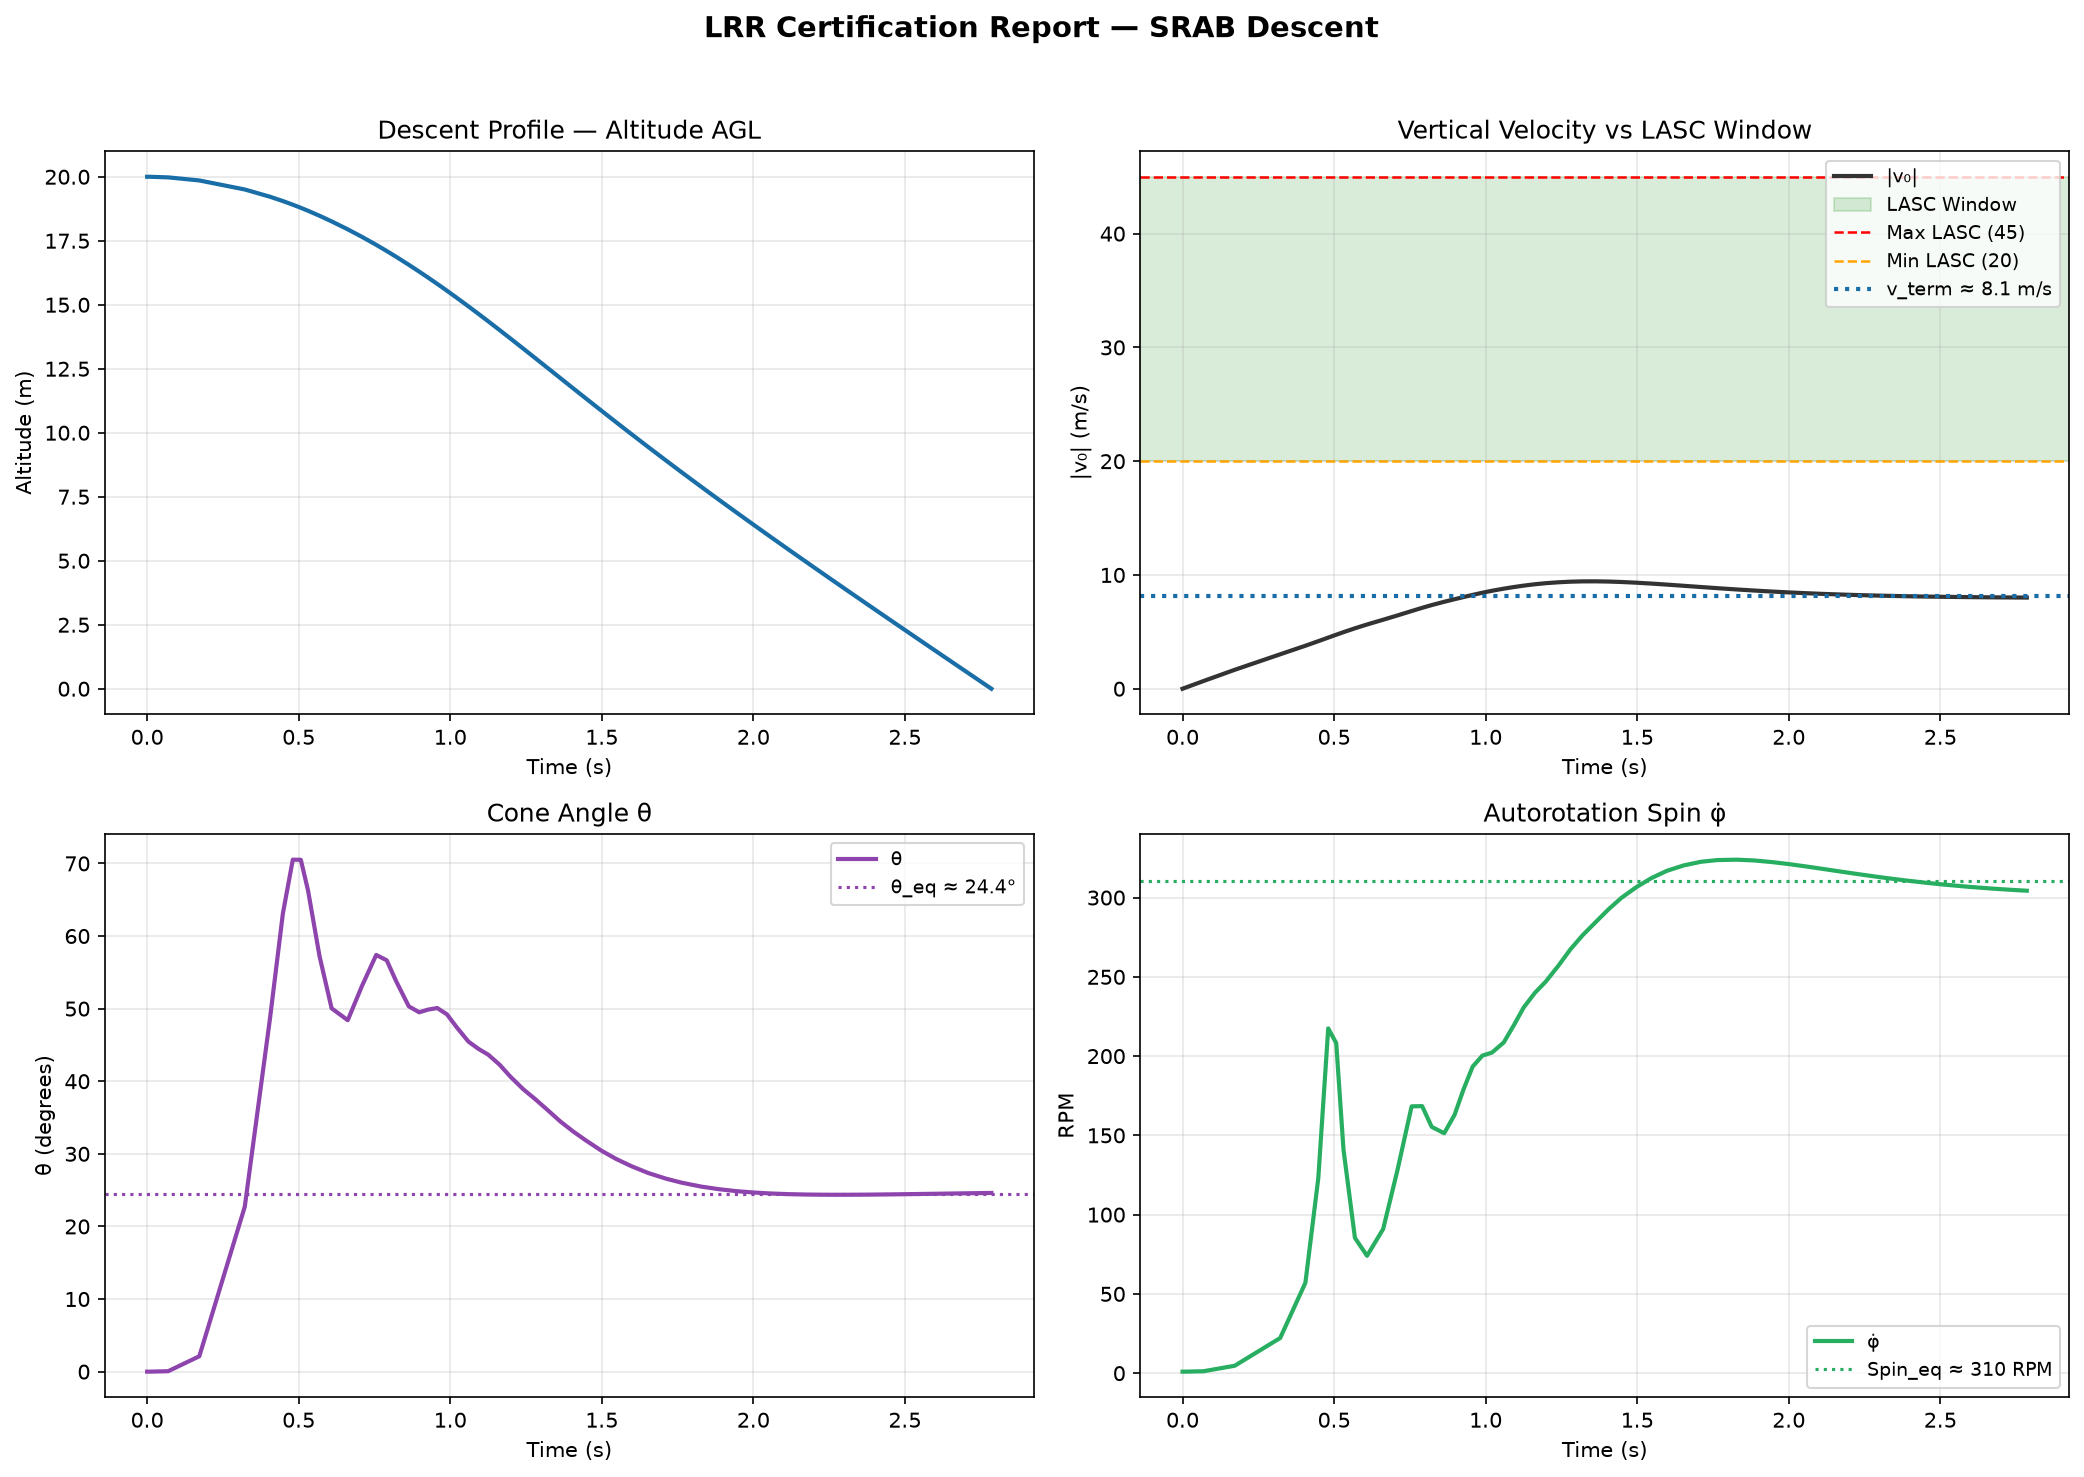
\includegraphics[width=0.9\textwidth]{figures/fig_test2_lrr.png}
\caption{LRR certification dashboard of Test~2 (Asa2, 4 wings, drone
drop from $\sim$20~m): the increased wing area (122.28~cm$^2$)
delivers a lower terminal velocity with a stable autorotation
state. The alpha-version onboard electronics were validated in this
drop, and the data confirmed the need for higher drop altitudes to
escape the transient regime.}
\label{fig:test2-lrr}
\end{figure}

Test~1 (Asa1, 4 wings) was the first time the samara autorotation
principle was observed in flight on the Helike project: the
prototype reached a stable coning motion within a fraction of a
second of release and the spin axis remained steady through the
descent, confirming that the deploy mechanism was passive and
deterministic. Test~2 (Asa2, 4 wings, wing area 122.28~cm$^2$)
increased the wing area by 12\% over Asa1 and was evaluated as the
intermediate candidate, reaching 8.04~m/s at impact with a stable
autorotation state; the same flight also carried the first
alpha-version onboard electronics, which recorded the rotation
profile with the flight IMU and produced the ENMC consolidated
dataset. The drone-altitude drops (Tests~1--2, $\sim$20~m) are too
short to reach the terminal velocity: the vehicle is still
accelerating at impact, so the measured values are transient and
must be compared against the simulated terminal values, not
directly against the LASC limit. The data from Tests~1--2 made it
clear that higher drop altitudes were required to leave the
transient regime, and Test~3 (Asa3, 4 wings, $\sim$30~m drone
drop, $\sim$200~g payload representative of the final assembly,
electronics onboard) was designed for exactly that --- the higher
release altitude and the realistic mass moved the impact point
closer to the steady autorotation regime. The same flight also
validated the onboard electronics, with the SRAB instrumented to
record rotation with the flight IMU (ENMC consolidated data).

\subsubsection{Geometry Comparison and Final Choice}

A comparative simulation of Asa2 (4 wings) vs. Asa3 (2 wings) showed
8.04 vs. 13.33~m/s terminal velocity after the radius optimization.
The Asa3 2-wing configuration (optimized aerodynamic radius
79.7~mm) was chosen as the final configuration for the mission: it
reaches the 20/1.5~m/s design target with a 1.5 safety factor on the
LASC 20~m/s limit, while offering lower mass and complexity than the
4-wing versions.

The choice between four and two wings is a direct trade-off between
redundancy and simplicity. The 4-wing variants (Asa1, Asa2) provide
geometric redundancy --- a single lost wing degrades performance
without preventing autorotation --- and a lower terminal velocity,
which increases the margin against the 20~m/s limit. However, they pay
for this in mass, rotating inertia and mechanical
complexity: each additional wing adds 3D-printed material, bonding
area and a potential failure surface, and the higher rotating mass
stores more kinetic energy at impact for the same descent velocity.
The 2-wing Asa3 exploits the same autorotation physics with roughly
half the wing area (58.7~cm$^2$ vs. 122.28~cm$^2$) and, being
lighter, spins faster at equilibrium (477~rpm vs. 372~rpm for the
4-wing test geometry), which increases the gyroscopic stiffness that
stabilizes the coning motion. At the cost of reduced geometric
redundancy, it still sits 1.5$\times$ below the regulatory limit, and
the drop-test evidence (Tests 1--3) confirms that deployment and
steady autorotation are deterministic with the passive geometry ---
there are no hinges or actuators to jam, so the redundancy argument
that motivates four wings is largely addressed by the mechanism's
inherent robustness rather than by part count. The mission risk
assessment (Appendix B) treats single-wing loss as a degraded-mode
event bounded by the same 20~m/s limit, and the mechanical
simplification of two wings directly supports the schedule-driven
development goal of the project.

% TODO: Test 4 (~200 m drop) is the next step for quantitative
% aerodynamic validation of the Asa3 2-wing configuration.
